% =====================================================================
\partieENO{Le circuit d'eau}

Cette partie décrit comment l'eau circule dans la tour et ce que cela donne en chiffres. Je commence par le principe du circuit et par la difficulté qui a fait naître la pièce la plus particulière de la tour, le couvercle répartiteur. Je donne ensuite ses dimensions, puis je calcule le débit que la pompe fournit vraiment dans ce circuit. J'en déduis ce que reçoit chaque plant, la vitesse à laquelle le bac se renouvelle et la fréquence à laquelle il faut refaire le plein. Je compare ensuite les besoins en eau et en nutriments des plantes, au cours de leur vie, à la littérature, et je justifie pourquoi je n'ajoute pas de bac de secours. Je termine par le protocole de mesure, car aucune mesure n'est encore faite : tous les chiffres de cette partie sont théoriques.

\subsection{Le principe du circuit et la difficulté de départ}

La tour est un tube de PVC vertical de \qty{1}{m}, de diamètre intérieur \qty{144}{mm} et de diamètre extérieur \qty{159}{mm}. Il porte 12 plants de laitue. Une pompe immergée dans le bac de \qty{152}{L} envoie l'eau en haut de la tour par un tuyau flexible de \qty{9}{mm} de diamètre intérieur. L'eau y est répartie, elle ruisselle le long de la paroi, mouille les racines, puis retombe dans le bac par gravité. Le circuit est fermé : l'eau tourne en boucle et ne se perd que par la consommation des plantes et par l'évaporation. Le schéma hydraulique de la page suivante résume l'ensemble : bac, pompe, tour, dosage, sondes et appoint.

\schemapaysageC{Schema_hydraulique_hydroponie.pdf}{hydro}{Schéma hydraulique de la tour : bac unique, pompe de circulation -M1, pompes de dosage -M2 à -M4, sondes -B1 à -B4 et appoint manuel.}

Mon premier problème est la répartition. Si le tuyau débouche simplement en haut du tube, l'eau tombe en un jet central et suit le même chemin à chaque fois : les racines placées au bord ne sont presque pas mouillées, et celles du centre sont noyées. Il faut une pièce qui répartisse l'eau sur toute la circonférence du tube. J'ai donc conçu un couvercle répartiteur, imprimé en 3D, qui joue le rôle d'une pomme de douche.

\subsection{Le couvercle répartiteur}

Le couvercle se pose sur le haut du tube. Son embase s'emboîte dans le tube (diamètre \qty{144}{mm}, égal au diamètre intérieur du PVC) et sa bride de \qty{168}{mm} de diamètre recouvre la tranche du tube, qui fait \qty{159}{mm} à l'extérieur. L'eau arrive par un moyeu central de \qty{44}{mm}. Elle est ensuite guidée par \textbf{huit canaux} disposés en étoile, à \ang{45} les uns des autres, jusqu'à \textbf{huit trous de \qty{4}{mm} de diamètre} percés vers la paroi du tube. Chaque canal alimente un trou : l'eau sort donc en huit points régulièrement espacés et se répartit sur toute la circonférence.

Le plan du couvercle répartiteur, reproduit ci-dessous, donne ses dimensions et la position des huit canaux.

\begin{figure}[H]
\centering
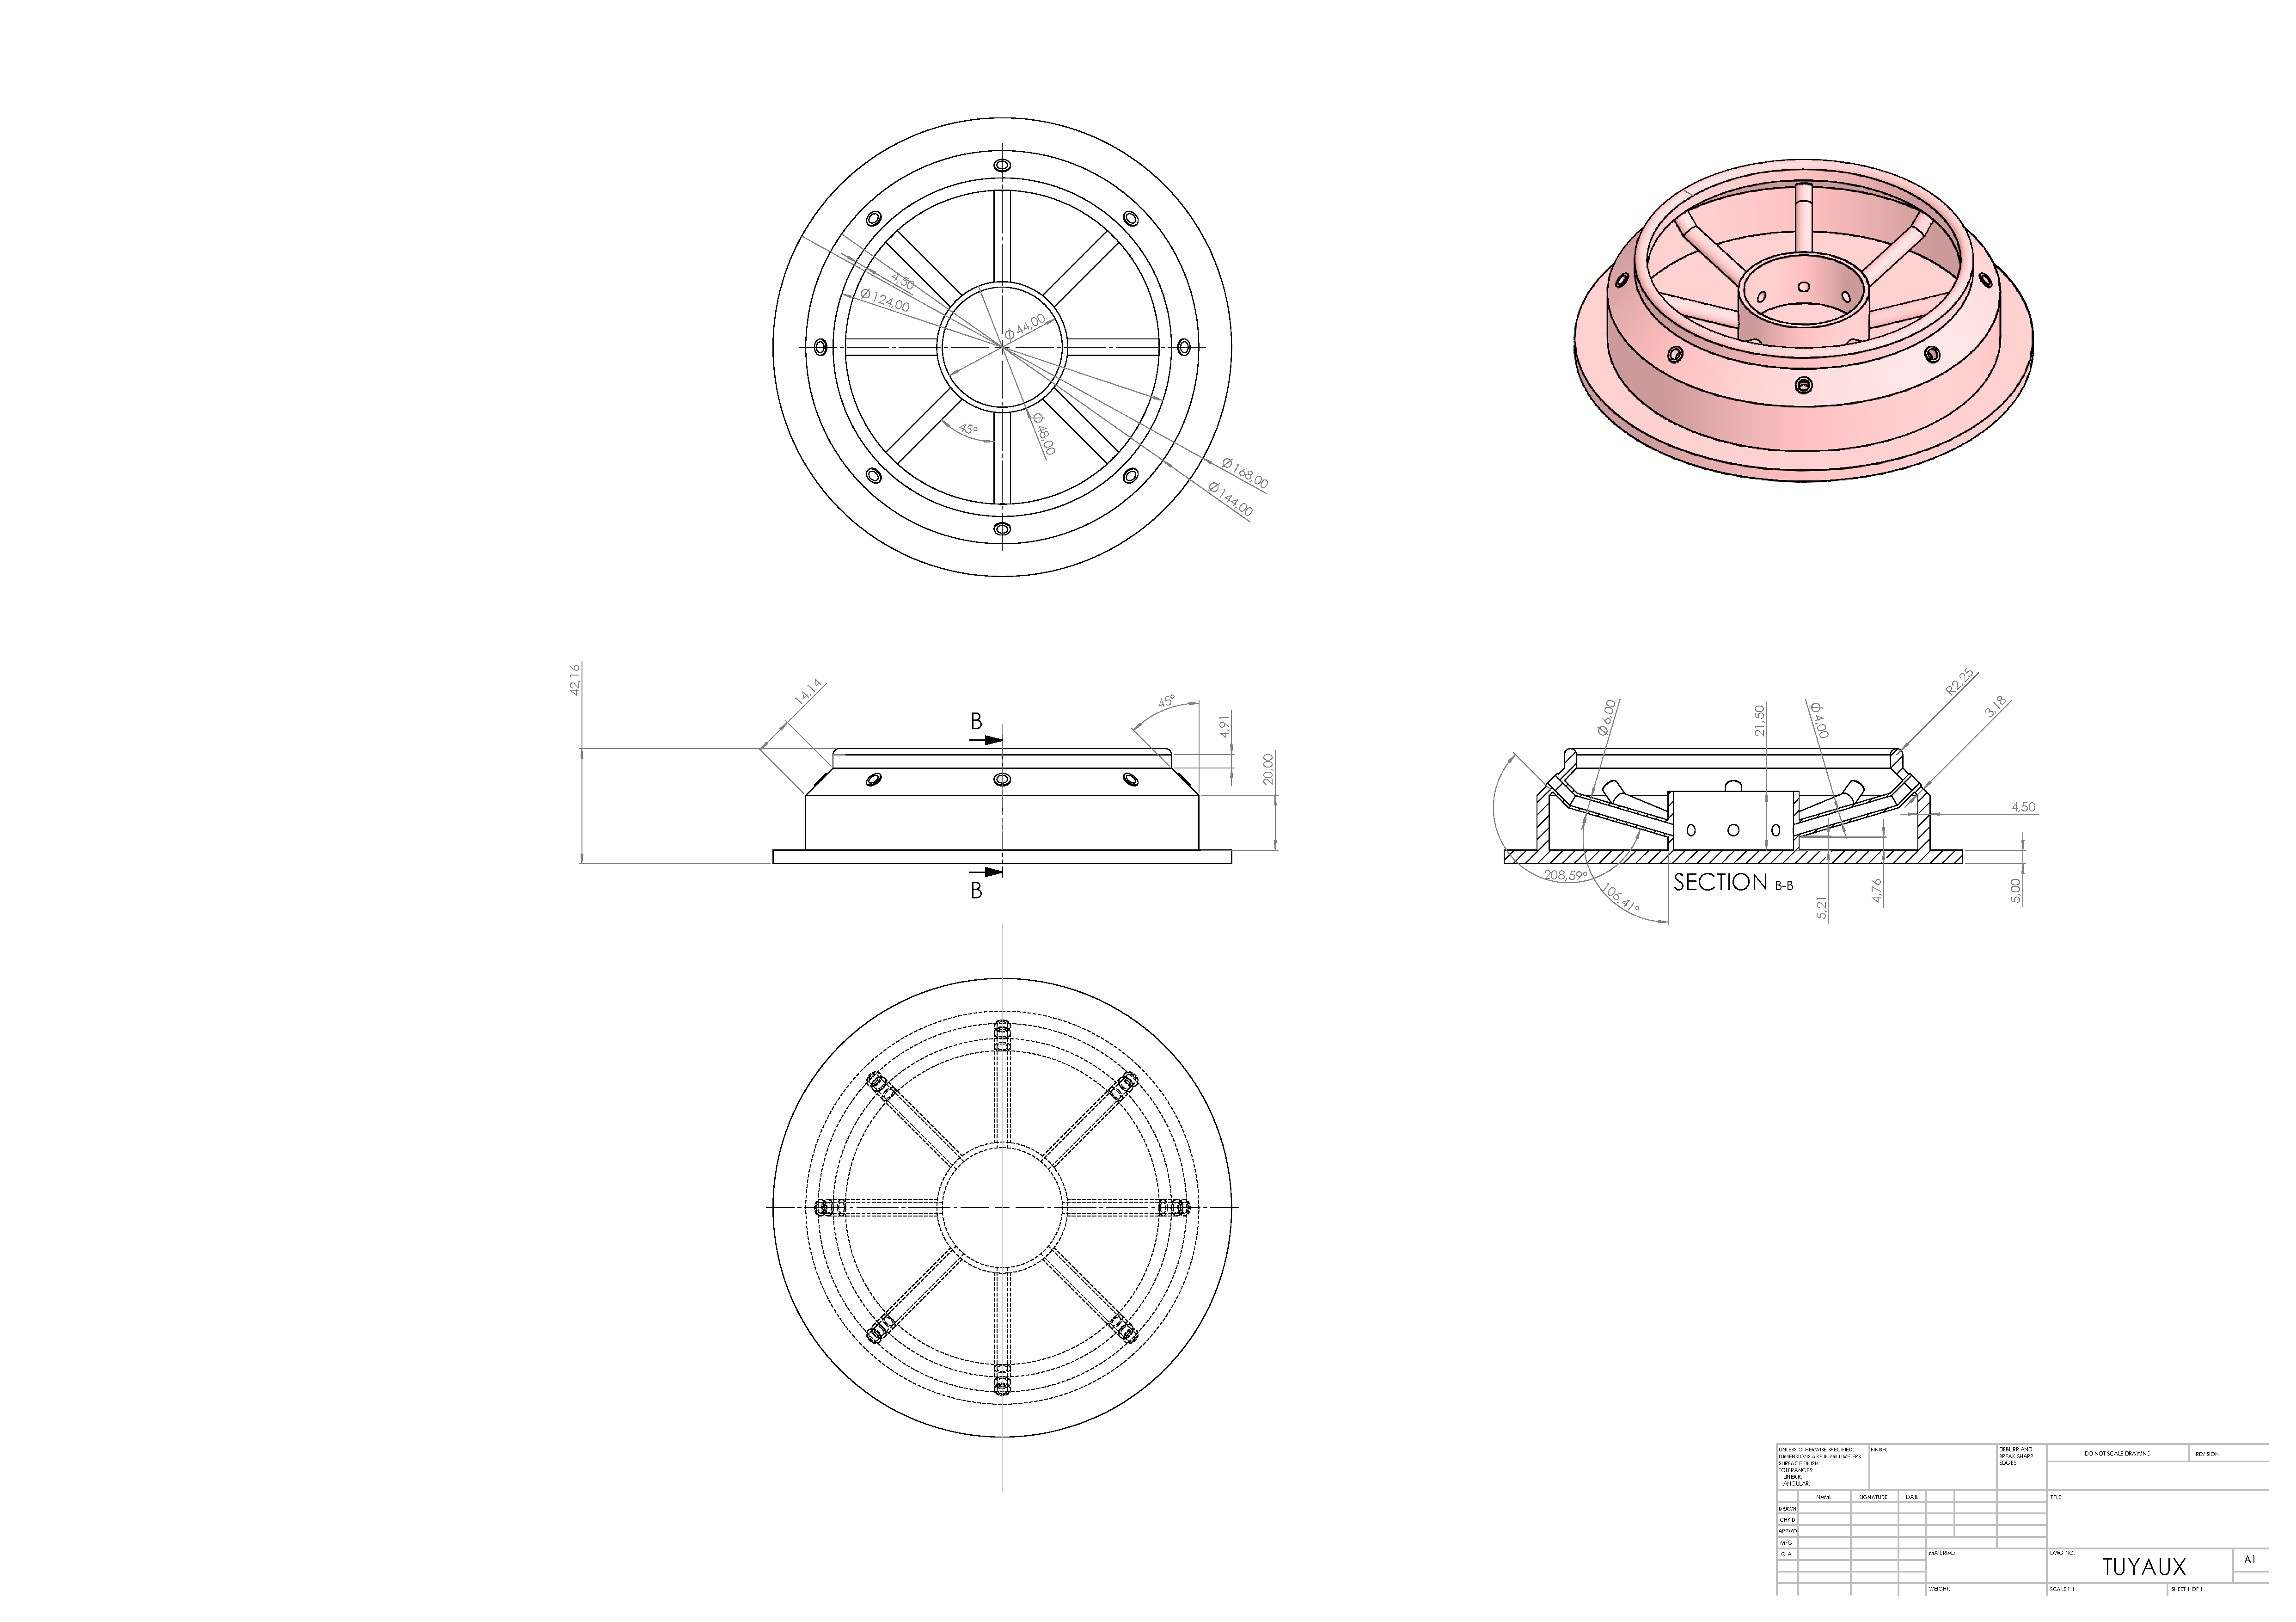
\includegraphics[page=1,trim=763bp 50bp 30bp 118bp,clip,width=0.86\textwidth]{Plan_couvercle_repartiteur.pdf}
\schemacap{planrep}{Plan du couvercle répartiteur : vue de dessus, vue de côté, vue de dessous avec les huit canaux et coupe B-B.}
\end{figure}

Le plan du couvercle répartiteur est la figure ci-dessus. Le plan de la pièce COUVERCLE (bouchon et embout) est reproduit en pleine page ci-dessous. Les deux plans complets sont aussi dans les annexes 1 et 2, à la fin du rapport.

\schemapaysageC[page=1]{Plan_couvercle_bouchon.pdf}{planbou}{Plan de la pièce COUVERCLE (bouchon et embout).}

Le choix du nombre de trous est un compromis. Plus il y en a, mieux l'eau est répartie, mais plus ils sont petits et plus ils risquent de se boucher avec les dépôts d'engrais. Huit trous de \qty{4}{mm} sont assez gros pour rester ouverts et assez nombreux pour que chaque trou arrose environ un huitième de la paroi, soit une zone d'environ \qty{57}{mm} de large sur le périmètre intérieur de \qty{452}{mm}.

\naturecalc{théorie, avec les dimensions mesurées sur la tour (bac, flexible, tube) et des valeurs de fiches techniques ; aucun débit ni aucune consommation n'est mesuré}
\begin{demonstration}[périmètre arrosé par chaque trou]
\resultat{p \approx \qty{57}{mm}}
Je note $D_t$ le diamètre intérieur du tube de la tour, en mètres (ici \qty{0,144}{m}), $P$ le périmètre intérieur du tube, en mètres, $n$ le nombre de trous (sans unité) et $p$ la longueur de paroi arrosée par un trou, en mètres. Le périmètre d'un cercle vaut $\pi$ fois son diamètre :
\begin{align*}
P &= \pi\, D_t\\
P &= \pi \times \qty{0,144}{m}\\
P &\approx \qty{0,452}{m}
\end{align*}
J'arrondis à trois chiffres. Les huit trous sont régulièrement espacés, donc chacun arrose la même longueur :
\begin{align*}
p &= \frac{P}{n}\\
p &= \frac{\qty{0,452}{m}}{8}\\
p &\approx \qty{0,0565}{m}
\end{align*}
soit environ \qty{57}{mm}, en arrondissant au millimètre.
\end{demonstration}

\subsection{Le point de fonctionnement de la pompe}

\subsubsection*{Ce que je cherche et ce que je suppose}

Je cherche le débit que la pompe fournit réellement dans ce circuit. La fiche de la pompe ne donne que deux points : à débit nul, elle monte l'eau à $H_{max} = \qty{5}{m}$ ; sans hauteur à vaincre, elle débite $Q_{max} = \qty{800}{L/h}$. Pour connaître le débit réel, je compare ce que la pompe peut fournir à ce que le circuit demande : le débit réel est celui pour lequel les deux hauteurs sont égales.

Faute de courbe constructeur, je relie les deux points connus par une droite. Je ne connais que ces deux points : je ne peux donc pas savoir de quel côté de la droite passe la vraie courbe de la pompe. Le débit de \qty{388}{L/h} est un résultat théorique, valable sous l'hypothèse de la droite, et non un débit garanti. Je le remplacerai par la mesure décrite dans le protocole, faite avec le circuit complet.

Les données du circuit sont les suivantes. Certaines sont mesurées, d'autres sont des hypothèses à vérifier.

\begin{table}[H]
\centering
\small
\renewcommand{\arraystretch}{1.1}
\begin{tabularx}{\textwidth}{|>{\raggedright\arraybackslash}p{5.6cm}|Y|>{\raggedright\arraybackslash}p{2.6cm}|}
\hline
\textbf{Donnée} & \textbf{Valeur retenue} & \textbf{Statut} \\
\hline
Volume du bac & \qty{152}{L} & mesuré \\
\hline
Pompe de circulation & \qty{800}{L/h} maximum, \qty{5}{m} maximum, \qty{12}{V}, \qty{19}{W} & fiche technique \\
\hline
Marche de la pompe & \qty{6,75}{h} par jour : le jour (10 h, de 7 h à 17 h), \qty{15}{min} de marche puis \qty{15}{min} d'arrêt, soit \qty{5}{h} ; la nuit (14 h, de 17 h à 7 h), 7 marches de \qty{15}{min} (17 h, 17 h 30, 21 h, 0 h, 3 h, 6 h et 6 h 30) $= \qty{1,75}{h}$ ; la coupure jour/nuit est choisie ici pour le bilan hydraulique, et la partie 5 la place à 6 h et 18 h, pour le même total & choix du projet \\
\hline
Diamètre intérieur du flexible & \qty{9}{mm} & mesuré \\
\hline
Longueur du flexible & \qty{1,8}{m} (\qty{0,4}{m} dans le bac, \qty{1,0}{m} le long de la tour, \qty{0,4}{m} de raccord) & hypothèse \\
\hline
Hauteur entre la surface du bac et le couvercle & \qty{1,2}{m} & hypothèse \\
\hline
Trous du couvercle & 8 trous de \qty{4}{mm} & plan \\
\hline
Pertes singulières & somme des coefficients $K = 2,8$ & hypothèse \\
\hline
Contraction du jet à la sortie d'un trou & coefficient $C_d = 0,62$ & hypothèse \\
\hline
Eau à \qty{25}{\celsius} & masse volumique \qty{997}{kg/m^3}, viscosité cinématique \qty{0,893e-6}{m^2/s} & tables \\
\hline
\end{tabularx}
\caption{Données du circuit d'eau.}
\end{table}

Les pertes singulières regroupent l'entrée dans la pompe et le raccord (coefficient \num{0,5}), deux coudes à \ang{90} (\num{0,9} chacun) et l'entrée dans le couvercle (\num{0,5}), soit $K = 0,5 + 2 \times 0,9 + 0,5 = 2,8$.

\subsubsection*{La courbe de la pompe}

\naturecalc{théorie, avec les dimensions mesurées sur la tour (bac, flexible, tube) et des valeurs de fiches techniques ; aucun débit ni aucune consommation n'est mesuré}
\begin{demonstration}[courbe linéaire de la pompe]
\resultat{H_p(Q) = H_{max}\left(1 - \dfrac{Q}{Q_{max}}\right)}
Je note $Q$ le débit de la pompe, en litres par heure, et $H_p$ la hauteur d'eau qu'elle peut fournir à ce débit, en mètres. Je cherche une droite de la forme :
\begin{align*}
H_p(Q) &= \alpha\,Q + \beta
\end{align*}
où $\alpha$ est sa pente, en mètres par litre par heure, et $\beta$ son ordonnée à l'origine, en mètres. Elle passe par le point $(Q = 0\,;\,H_p = H_{max})$. En remplaçant $Q$ par $0$ :
\begin{align*}
H_p(0) &= \alpha \times 0 + \beta\\
H_{max} &= \beta
\end{align*}
Elle passe aussi par le point $(Q = Q_{max}\,;\,H_p = 0)$. En remplaçant :
\begin{align*}
0 &= \alpha\, Q_{max} + H_{max}\\
\alpha\, Q_{max} &= -H_{max}\\
\alpha &= -\frac{H_{max}}{Q_{max}}
\end{align*}
En remettant $\alpha$ et $\beta$ dans l'équation de la droite :
\begin{align*}
H_p(Q) &= -\frac{H_{max}}{Q_{max}}\,Q + H_{max}\\
H_p(Q) &= H_{max}\left(1 - \frac{Q}{Q_{max}}\right)
\end{align*}
Avec les valeurs de la fiche :
\begin{align*}
H_p(Q) &= \qty{5}{m}\times\left(1 - \frac{Q}{\qty{800}{L/h}}\right)
\end{align*}
\end{demonstration}

\subsubsection*{La courbe du circuit}

La courbe du circuit donne la hauteur que la pompe doit fournir pour faire passer un débit donné dans le tuyau et dans le couvercle. Je pars de la conservation de l'énergie de l'eau, puis j'ajoute les pertes.

\naturecalc{théorie, avec les dimensions mesurées sur la tour (bac, flexible, tube) et des valeurs de fiches techniques ; aucun débit ni aucune consommation n'est mesuré}
\begin{demonstration}[hauteur demandée par le circuit]
\resultat{H_r = H_g + \dfrac{v_j^2}{2g} + h_r + h_s}
Je considère une tranche d'eau de masse $m$, en kilogrammes, de volume $m/\rho$, avec $\rho$ la masse volumique de l'eau, en kilogrammes par mètre cube. Elle a trois énergies :
\begin{align*}
E_{pression} &= p\,\frac{m}{\rho}\\
E_{cin} &= \frac{1}{2}\,m\,v^2\\
E_{pot} &= m\,g\,z
\end{align*}
où $p$ est la pression, en pascals, $v$ la vitesse, en mètres par seconde, $g = \qty{9,81}{m/s^2}$ l'accélération de la pesanteur et $z$ l'altitude, en mètres. Je divise chaque énergie par le poids $m g$ de la tranche, en newtons : j'obtiens une énergie par unité de poids, qui s'exprime en mètres, donc une hauteur :
\begin{align*}
e &= \frac{p}{\rho g} + \frac{v^2}{2g} + z
\end{align*}
Entre la surface du bac (point 1) et la sortie des trous du couvercle (point 2), la pompe apporte la hauteur $H$, en mètres, et les frottements en retirent $\Delta H$, en mètres :
\begin{align*}
\frac{p_1}{\rho g} + \frac{v_1^2}{2g} + z_1 + H &= \frac{p_2}{\rho g} + \frac{v_2^2}{2g} + z_2 + \Delta H
\end{align*}
Au point 1, l'eau est à la pression atmosphérique $p_{atm}$ et presque immobile, car la surface du bac est très grande devant le tuyau : $p_1 = p_{atm}$ et $v_1 \approx 0$. Au point 2, l'eau sort à l'air libre : $p_2 = p_{atm}$, avec la vitesse de jet $v_j$. Les pressions atmosphériques s'annulent. En notant $H_g = z_2 - z_1$ la hauteur entre la surface du bac et le couvercle, en mètres :
\begin{align*}
H &= H_g + \frac{v_j^2}{2g} + \Delta H
\end{align*}
Les pertes se séparent en pertes régulières $h_r$ (frottement le long du tuyau) et pertes singulières $h_s$ (coudes, raccords), toutes en mètres :
\begin{align*}
\Delta H &= h_r + h_s
\end{align*}
La hauteur $H$ que la pompe doit fournir est la hauteur demandée par le circuit, notée $H_r$ :
\begin{align*}
H_r &= H_g + \frac{v_j^2}{2g} + h_r + h_s
\end{align*}
\end{demonstration}

\naturecalc{théorie, avec les dimensions mesurées sur la tour (bac, flexible, tube) et des valeurs de fiches techniques ; aucun débit ni aucune consommation n'est mesuré}
\begin{demonstration}[perte de charge régulière]
\resultat{h_r = \lambda\,\dfrac{L}{D}\,\dfrac{v^2}{2g}}
Je note $L$ la longueur du tuyau, en mètres, $D$ son diamètre intérieur, en mètres, et $v$ la vitesse moyenne de l'eau, en mètres par seconde. J'isole un tronçon de tuyau où l'écoulement est établi : la vitesse ne change pas, donc la quantité de mouvement de l'eau ne change pas et les forces se compensent. La différence de pression $\Delta p$, en pascals, sur les deux sections pousse l'eau ; la contrainte de frottement $\tau_p$, en pascals, sur la paroi la retient :
\begin{align*}
\Delta p \cdot \frac{\pi D^2}{4} &= \tau_p \cdot \pi D L
\end{align*}
Je divise les deux membres par $\pi D^2/4$ :
\begin{align*}
\Delta p &= \frac{4\,\tau_p\,L}{D}
\end{align*}
La contrainte $\tau_p$ dépend de $\rho$, de $v$ et de la viscosité. La seule grandeur homogène à une pression que l'on peut former avec $\rho$ et $v$ est $\rho v^2$. Le rapport $\tau_p/(\rho v^2)$ est donc un nombre sans dimension : il ne peut dépendre que du nombre de Reynolds $Re = vD/\nu$, avec $\nu$ la viscosité cinématique de l'eau, en mètres carrés par seconde. Je l'écris par convention $\lambda/8$, où $\lambda$ est le coefficient de frottement, sans unité :
\begin{align*}
\tau_p &= \frac{\lambda}{8}\,\rho v^2
\end{align*}
En remplaçant dans l'expression de $\Delta p$ :
\begin{align*}
\Delta p &= \frac{4 L}{D}\times\frac{\lambda}{8}\,\rho v^2\\
\Delta p &= \lambda\,\frac{L}{D}\,\frac{\rho v^2}{2}
\end{align*}
Pour l'exprimer en hauteur d'eau, je divise par $\rho g$ :
\begin{align*}
h_r &= \frac{\Delta p}{\rho g}\\
h_r &= \lambda\,\frac{L}{D}\,\frac{v^2}{2g}
\end{align*}
Pour un tuyau lisse en régime turbulent ($4000 < Re < 10^5$), la loi expérimentale que j'utilise pour $\lambda$ est :
\begin{align*}
\lambda &= 0,316\,Re^{-1/4}
\end{align*}
\end{demonstration}

\naturecalc{théorie, avec les dimensions mesurées sur la tour (bac, flexible, tube) et des valeurs de fiches techniques ; aucun débit ni aucune consommation n'est mesuré}
\begin{demonstration}[perte singulière, vitesse du tuyau et vitesse du jet]
\resultat{H_r(Q) = H_g + \left(\lambda\dfrac{L}{D} + K\right)\dfrac{Q^2}{2gA^2} + \dfrac{Q^2}{2g\,a^2}}
Chaque coude ou raccord dissipe une fraction de l'énergie cinétique de l'eau, proportionnelle à $v^2/(2g)$ par un coefficient $K_i$ propre à la pièce, sans unité. En additionnant toutes les pièces :
\begin{align*}
h_s &= \left(\sum K_i\right)\frac{v^2}{2g}\\
h_s &= K\,\frac{v^2}{2g}
\end{align*}
Le débit volumique $Q$, en mètres cubes par seconde, est le même dans toute section du tuyau. Avec $A$ la section intérieure du tuyau, en mètres carrés :
\begin{align*}
Q &= v\,A\\
v &= \frac{Q}{A}\\
A &= \frac{\pi D^2}{4}
\end{align*}
À la sortie de chaque trou de diamètre $d$, en mètres, le jet se contracte à la section $C_d\,\pi d^2/4$. Avec $n$ trous, la section utile totale $a$, en mètres carrés, vaut :
\begin{align*}
a &= n\,C_d\,\frac{\pi d^2}{4}
\end{align*}
et la vitesse du jet $v_j$, en mètres par seconde, vaut :
\begin{align*}
v_j &= \frac{Q}{a}
\end{align*}
Je remplace $h_r$, $h_s$, $v$ et $v_j$ dans $H_r$ :
\begin{align*}
H_r(Q) &= H_g + \left(\lambda\frac{L}{D} + K\right)\frac{v^2}{2g} + \frac{v_j^2}{2g}\\
H_r(Q) &= H_g + \left(\lambda\frac{L}{D} + K\right)\frac{Q^2}{2gA^2} + \frac{Q^2}{2g\,a^2}
\end{align*}
\end{demonstration}

\naturecalc{théorie, avec les dimensions mesurées sur la tour (bac, flexible, tube) et des valeurs de fiches techniques ; aucun débit ni aucune consommation n'est mesuré}
\begin{demonstration}[sections du tuyau et du couvercle]
\resultat{a \approx \qty{62,3}{mm^2}\ \text{pour}\ A \approx \qty{63,6}{mm^2}}
La section intérieure du flexible, de diamètre $D = \qty{9}{mm} = \qty{0,009}{m}$, vaut :
\begin{align*}
A &= \frac{\pi D^2}{4}\\
A &= \frac{\pi \times (\qty{0,009}{m})^2}{4}\\
A &\approx \qty{6,36e-5}{m^2}
\end{align*}
La section utile des huit trous de diamètre $d = \qty{4}{mm} = \qty{0,004}{m}$, avec $C_d = 0,62$, vaut :
\begin{align*}
a &= n\,C_d\,\frac{\pi d^2}{4}\\
a &= 8 \times 0,62 \times \frac{\pi \times (\qty{0,004}{m})^2}{4}\\
a &\approx \qty{6,23e-5}{m^2}
\end{align*}
Les deux sections sont presque égales (rapport $A/a \approx 1,02$) : le couvercle ne freine presque pas l'eau, il la répartit sans former un jet rapide.
\end{demonstration}

\subsubsection*{Le point de fonctionnement}

Le débit réel est celui pour lequel la hauteur fournie par la pompe égale la hauteur demandée par le circuit : $H_p(Q) = H_r(Q)$. Comme le coefficient $\lambda$ dépend lui-même du débit, je ne peux pas isoler $Q$ à la main : je résous l'équation numériquement avec un script. Je vérifie ensuite le résultat terme par terme.

La figure suivante superpose la courbe de la pompe et celle du circuit : leur croisement est le point de fonctionnement.

\begin{figure}[H]
\centering
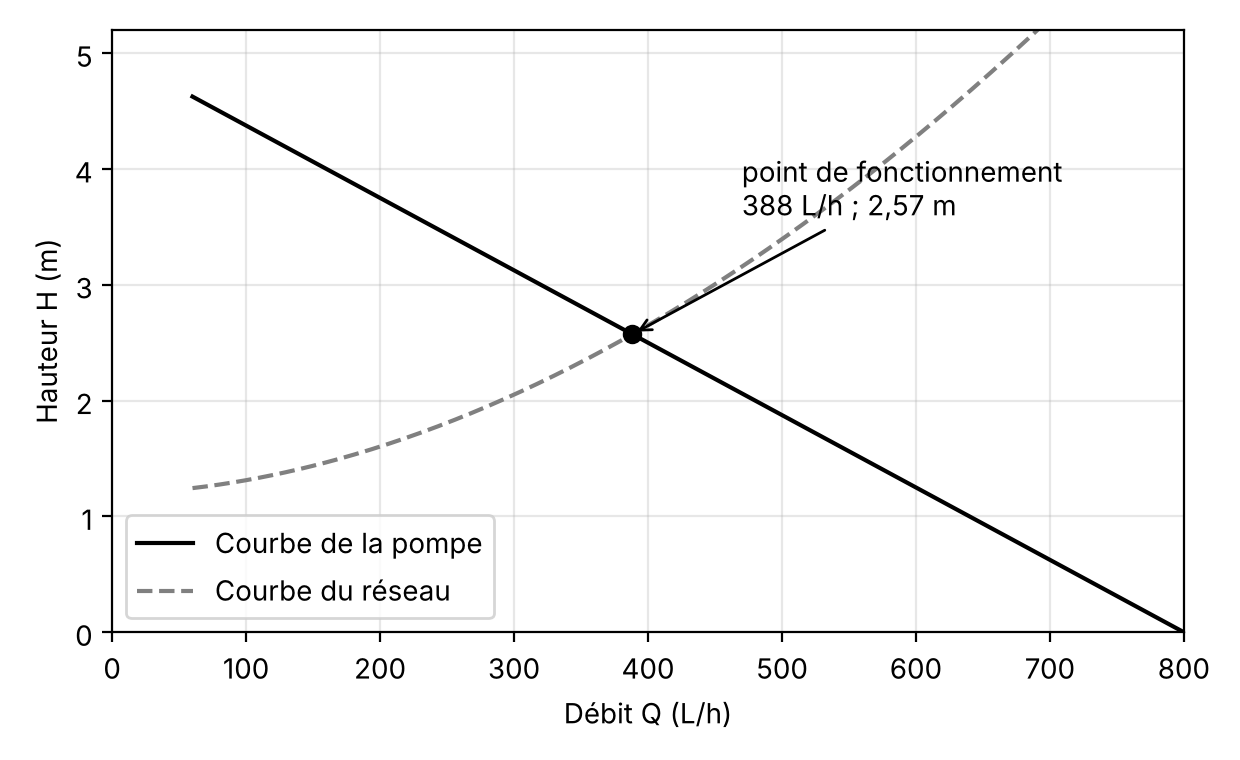
\includegraphics[width=0.82\textwidth]{img/point_fonct.png}
\caption{Courbe de la pompe, courbe du circuit et point de fonctionnement.}
\end{figure}

\naturecalc{théorie, avec les dimensions mesurées sur la tour (bac, flexible, tube) et des valeurs de fiches techniques ; aucun débit ni aucune consommation n'est mesuré}
\begin{demonstration}[vérification du point de fonctionnement]
\resultat{Q \approx \qty{388}{L/h}\ \text{sous}\ H \approx \qty{2,57}{m}}
Le script donne le débit $Q = \qty{1,0787e-4}{m^3/s}$. Je le convertis en litres par heure, sachant qu'un mètre cube vaut \qty{1000}{L} et qu'une heure vaut \qty{3600}{s} :
\begin{align*}
Q &= \qty{1,0787e-4}{m^3/s} \times \qty{1000}{L/m^3} \times \qty{3600}{s/h}\\
Q &\approx \qty{388,3}{L/h}
\end{align*}
La vitesse dans le tuyau vaut :
\begin{align*}
v &= \frac{Q}{A}\\
v &= \frac{\qty{1,0787e-4}{m^3/s}}{\qty{6,362e-5}{m^2}}\\
v &\approx \qty{1,696}{m/s}
\end{align*}
Le nombre de Reynolds vaut :
\begin{align*}
Re &= \frac{v\,D}{\nu}\\
Re &= \frac{\qty{1,696}{m/s}\times\qty{0,009}{m}}{\qty{0,893e-6}{m^2/s}}\\
Re &\approx 17\,100
\end{align*}
Ce nombre est supérieur à $4000$ : l'écoulement est turbulent et la loi de $\lambda$ s'applique.
\begin{align*}
\lambda &= 0,316 \times 17\,089^{-1/4}\\
\lambda &= \frac{0,316}{11,43}\\
\lambda &\approx 0,0276
\end{align*}
L'énergie cinétique par unité de poids dans le tuyau vaut :
\begin{align*}
\frac{v^2}{2g} &= \frac{(\qty{1,696}{m/s})^2}{2\times\qty{9,81}{m/s^2}}\\
\frac{v^2}{2g} &\approx \qty{0,1465}{m}
\end{align*}
Le rapport $L/D$ vaut $\qty{1,8}{m}/\qty{0,009}{m} = 200$. Les pertes régulières valent :
\begin{align*}
h_r &= 0,0276 \times 200 \times \qty{0,1465}{m}\\
h_r &\approx \qty{0,810}{m}
\end{align*}
Les pertes singulières valent :
\begin{align*}
h_s &= 2,8 \times \qty{0,1465}{m}\\
h_s &\approx \qty{0,410}{m}
\end{align*}
La vitesse du jet vaut :
\begin{align*}
v_j &= \frac{Q}{a}\\
v_j &= \frac{\qty{1,0787e-4}{m^3/s}}{\qty{6,233e-5}{m^2}}\\
v_j &\approx \qty{1,731}{m/s}
\end{align*}
et son énergie cinétique par unité de poids :
\begin{align*}
\frac{v_j^2}{2g} &= \frac{(\qty{1,731}{m/s})^2}{2\times\qty{9,81}{m/s^2}}\\
\frac{v_j^2}{2g} &\approx \qty{0,153}{m}
\end{align*}
La hauteur demandée par le circuit vaut :
\begin{align*}
H_r &= \qty{1,2}{m} + \qty{0,810}{m} + \qty{0,410}{m} + \qty{0,153}{m}\\
H_r &\approx \qty{2,573}{m}
\end{align*}
La hauteur fournie par la pompe vaut :
\begin{align*}
H_p &= \qty{5}{m}\times\left(1 - \frac{\qty{388,3}{L/h}}{\qty{800}{L/h}}\right)\\
H_p &= \qty{5}{m}\times 0,5146\\
H_p &\approx \qty{2,573}{m}
\end{align*}
Les deux hauteurs sont égales : le point de fonctionnement est vérifié. Les pertes dans le flexible ($h_r + h_s$, soit \qty{1,22}{m}) pèsent presque autant que la montée elle-même (\qty{1,2}{m}) : c'est le flexible fin de \qty{9}{mm} qui limite le débit, et non le couvercle.
\end{demonstration}

\naturecalc{théorie, avec les dimensions mesurées sur la tour (bac, flexible, tube) et des valeurs de fiches techniques ; aucun débit ni aucune consommation n'est mesuré}
\begin{demonstration}[pression avant le couvercle et hauteur du jet]
\resultat{p - p_{atm} \approx \qty{60}{Pa}\ \text{et}\ h_{jet} \approx \qty{15}{cm}}
Entre le tuyau juste avant le couvercle (vitesse $v$, pression $p$) et le jet (vitesse $v_j$, pression atmosphérique), à la même altitude et sans perte (déjà comptée par $C_d$), la conservation de l'énergie donne :
\begin{align*}
\frac{p - p_{atm}}{\rho g} + \frac{v^2}{2g} &= \frac{v_j^2}{2g}
\end{align*}
Je multiplie par $\rho g$ et j'isole la surpression, en pascals :
\begin{align*}
p - p_{atm} &= \frac{\rho}{2}\left(v_j^2 - v^2\right)\\
p - p_{atm} &= \frac{\qty{997}{kg/m^3}}{2}\times\left((\qty{1,731}{m/s})^2 - (\qty{1,696}{m/s})^2\right)\\
p - p_{atm} &\approx \qty{60}{Pa}
\end{align*}
soit environ $\qty{0,0006}{bar}$ : l'eau arrive presque sans pression au couvercle.

Si un trou était dirigé vers le haut, son jet monterait, sans frottement de l'air, jusqu'à ce que toute son énergie cinétique soit devenue potentielle :
\begin{align*}
\frac{1}{2}\,m\,v_j^2 &= m\,g\,h_{jet}\\
h_{jet} &= \frac{v_j^2}{2g}\\
h_{jet} &\approx \qty{0,153}{m}
\end{align*}
soit environ \qty{15}{cm}. Cette hauteur se mesure facilement et permet de vérifier le débit (protocole en fin de partie).
\end{demonstration}

\naturecalc{théorie, avec les dimensions mesurées sur la tour (bac, flexible, tube) et des valeurs de fiches techniques ; aucun débit ni aucune consommation n'est mesuré}
\begin{demonstration}[puissance hydraulique et rendement]
\resultat{P_h \approx \qty{2,7}{W}\ \text{et}\ \eta \approx 0,14}
La pompe élève chaque seconde un volume $Q$, c'est-à-dire un poids $\rho g Q$, en newtons par seconde, d'une hauteur $H$. Sa puissance hydraulique $P_h$, en watts, vaut donc :
\begin{align*}
P_h &= \rho\,g\,Q\,H\\
P_h &= \qty{997}{kg/m^3}\times\qty{9,81}{m/s^2}\times\qty{1,0787e-4}{m^3/s}\times\qty{2,573}{m}\\
P_h &\approx \qty{2,71}{W}
\end{align*}
Comparée aux $P_e = \qty{19}{W}$ électriques de la pompe, le rendement global $\eta$ (sans unité) vaut :
\begin{align*}
\eta &= \frac{P_h}{P_e}\\
\eta &= \frac{\qty{2,71}{W}}{\qty{19}{W}}\\
\eta &\approx 0,14
\end{align*}
Ce rendement faible est normal pour une petite pompe utilisée loin de son point de meilleur rendement. Il ne change pas la consommation électrique retenue dans l'étude énergétique, \qty{19}{W}.
\end{demonstration}

\subsubsection*{Sensibilité au diamètre du flexible}

Le diamètre du flexible est la donnée qui pèse le plus. Le tableau donne le point de fonctionnement pour d'autres flexibles courants, avec le même couvercle et la même longueur.

\begin{table}[H]
\centering
\small
\renewcommand{\arraystretch}{1.1}
\begin{tabularx}{\textwidth}{|Y|Y|Y|Y|}
\hline
\textbf{Diamètre intérieur (mm)} & \textbf{Débit (L/h)} & \textbf{Vitesse (m/s)} & \textbf{Hauteur (m)} \\
\hline
\textbf{9 (mon flexible)} & \textbf{388} & \textbf{1,70} & \textbf{2,57} \\
\hline
10 & 431 & 1,52 & 2,31 \\
\hline
13 & 505 & 1,06 & 1,84 \\
\hline
16 & 535 & 0,74 & 1,66 \\
\hline
\end{tabularx}
\caption{Point de fonctionnement selon le diamètre du flexible.}
\end{table}

Un flexible plus gros augmenterait le débit d'environ 30 \% (de \qty{388}{L/h} à \qty{505}{L/h} pour \qty{13}{mm}). Ce n'est pas nécessaire : on verra que \qty{388}{L/h} suffisent largement.

\subsection{Débit par plant et renouvellement du bac}

\naturecalc{théorie, avec les dimensions mesurées sur la tour (bac, flexible, tube) et des valeurs de fiches techniques ; aucun débit ni aucune consommation n'est mesuré}
\begin{demonstration}[débit par plant]
\resultat{q_{plant} \approx \qty{32}{L/h}}
Je note $n_p = 12$ le nombre de plants. Le couvercle répartit le débit $Q$ sur toute la paroi, donc chaque plant reçoit en moyenne :
\begin{align*}
q_{plant} &= \frac{Q}{n_p}\\
q_{plant} &= \frac{\qty{388,3}{L/h}}{12}\\
q_{plant} &\approx \qty{32,4}{L/h}
\end{align*}
soit \qty{0,54}{L/min}. Pour une tour à ruissellement, je retiens un besoin minimal de \qty{2}{L/h} par godet pendant la marche, pour que la paroi et les racines restent mouillées sur toute la hauteur. Le débit disponible est donc environ 16 fois supérieur à ce besoin :
\begin{align*}
\frac{q_{plant}}{q_{min}} &= \frac{\qty{32,4}{L/h}}{\qty{2}{L/h}}\\
\frac{q_{plant}}{q_{min}} &\approx 16
\end{align*}
\end{demonstration}

Cette division suppose une répartition égale, ce que le couvercle ne garantit pas : il n'a que 8 sorties pour 12 emplacements. Le débit moyen par sortie vaut $q_{trou} = \qty{388,3}{L/h} / 8 \approx \qty{48,5}{L/h}$. L'eau ruisselle ensuite le long de la paroi et peut mouiller plusieurs godets, mais je ne peux pas annoncer un débit réel par plant tant que la répartition n'est pas mesurée. Je retiens donc le débit moyen de \qty{32}{L/h} par plant comme un ordre de grandeur, et le vrai critère reste visuel : les huit zones arrosées doivent se rejoindre et toutes les racines doivent être mouillées pendant la marche. Ce sera vérifié à l'essai.

\naturecalc{théorie, avec les dimensions mesurées sur la tour (bac, flexible, tube) et des valeurs de fiches techniques ; aucun débit ni aucune consommation n'est mesuré}
\begin{demonstration}[temps de renouvellement du bac]
\resultat{\tau \approx \qty{23,5}{min}}
Le temps de renouvellement $\tau$ est la durée pour que la pompe fasse passer dans la tour un volume égal à celui du bac $V = \qty{152}{L}$ :
\begin{align*}
\tau &= \frac{V}{Q}\\
\tau &= \frac{\qty{152}{L}}{\qty{388,3}{L/h}}\\
\tau &\approx \qty{0,391}{h}
\end{align*}
Je multiplie par \qty{60}{min/h} :
\begin{align*}
\tau &= \qty{0,391}{h}\times\qty{60}{min/h}\\
\tau &\approx \qty{23,5}{min}
\end{align*}
Pendant les $t_{marche} = \qty{6,75}{h}$ de marche par jour, le volume du bac passe dans la tour :
\begin{align*}
N_j &= \frac{Q\,t_{marche}}{V}\\
N_j &= \frac{\qty{388,3}{L/h}\times\qty{6,75}{h/j}}{\qty{152}{L}}\\
N_j &= \frac{\qty{2621}{L/j}}{\qty{152}{L}}\\
N_j &\approx 17{,}2\ \text{fois par jour}
\end{align*}
Une période de marche de \qty{15}{min} fait donc passer environ $\qty{15}{min}/\qty{23,5}{min} \approx 64\ \%$ du volume du bac dans la tour.
\end{demonstration}

\subsection{Consommation d'eau et fréquence de l'appoint}

L'eau quitte le bac de deux façons : elle est absorbée par les plants (transpirée par les feuilles) et elle s'évapore au contact de l'air. Les chiffres suivants sont des hypothèses de départ, à remplacer par les mesures.

\begin{table}[H]
\centering
\small
\renewcommand{\arraystretch}{1.1}
\begin{tabularx}{\textwidth}{|>{\raggedright\arraybackslash}p{5.2cm}|Y|}
\hline
\textbf{Hypothèse} & \textbf{Valeur retenue} \\
\hline
Consommation d'une laitue adulte (pointe) & \qty{0,30}{L/j} par plant, pendant les 10 derniers jours avant la récolte \\
\hline
Consommation moyenne sur le cycle & \qty{0,15}{L/j} par plant : une laitue a peu de feuilles la première moitié du cycle, puis consomme de plus en plus, d'où une moyenne d'environ la moitié de la pointe \\
\hline
Évaporation & surface d'eau libre de \qty{0,10}{m^2} (ouvertures, godets, parois mouillées) et \qty{5}{mm/j}, eau tiède et air chaud et humide \\
\hline
Bac plein & bac de \qty{0,70}{m} sur \qty{0,45}{m}, soit une surface $S_{bac} = \qty{0,70}{m}\times\qty{0,45}{m} \approx \qty{0,315}{m^2}$, rempli avec \qty{152}{L} (hauteur d'eau $\qty{0,152}{m^3}/\qty{0,315}{m^2} \approx \qty{0,48}{m}$, bac plein) \\
\hline
Appoint toléré & baisse de 10 \% du volume du bac \\
\hline
\end{tabularx}
\caption{Hypothèses du bilan hydrique.}
\end{table}

\naturecalc{théorie, avec les dimensions mesurées sur la tour (bac, flexible, tube) et des valeurs de fiches techniques ; aucun débit ni aucune consommation n'est mesuré}
\begin{demonstration}[évaporation et consommation journalière]
\resultat{C_{pic} = \qty{4,1}{L/j}\ \text{et}\ C_{moy} = \qty{2,3}{L/j}}
Une lame d'eau de \qty{1}{mm} d'épaisseur sur \qty{1}{m^2} représente un volume de :
\begin{align*}
\qty{e-3}{m}\times\qty{1}{m^2} &= \qty{e-3}{m^3}\\
&= \qty{1}{L}
\end{align*}
Je note $S_e = \qty{0,10}{m^2}$ la surface d'eau libre et $e = \qty{5}{mm/j}$ la hauteur évaporée par jour. L'évaporation $E$, en litres par jour, vaut :
\begin{align*}
E &= S_e \times e \times \qty{1}{L/(mm\cdot m^2)}\\
E &= \qty{0,10}{m^2}\times\qty{5}{mm/j}\times\qty{1}{L/(mm\cdot m^2)}\\
E &= \qty{0,5}{L/j}
\end{align*}
La consommation journalière $C$ du bac, en litres par jour, est la somme de ce que boivent les $n_p$ plants (chacun $c$, en litres par jour) et de l'évaporation :
\begin{align*}
C &= n_p\,c + E
\end{align*}
En pointe ($c = \qty{0,30}{L/j}$) :
\begin{align*}
C_{pic} &= 12\times\qty{0,30}{L/j} + \qty{0,5}{L/j}\\
C_{pic} &= \qty{3,6}{L/j} + \qty{0,5}{L/j}\\
C_{pic} &= \qty{4,1}{L/j}
\end{align*}
En moyenne sur le cycle ($c = \qty{0,15}{L/j}$) :
\begin{align*}
C_{moy} &= 12\times\qty{0,15}{L/j} + \qty{0,5}{L/j}\\
C_{moy} &= \qty{1,8}{L/j} + \qty{0,5}{L/j}\\
C_{moy} &= \qty{2,3}{L/j}
\end{align*}
\end{demonstration}

\naturecalc{théorie, avec les dimensions mesurées sur la tour (bac, flexible, tube) et des valeurs de fiches techniques ; aucun débit ni aucune consommation n'est mesuré}
\begin{demonstration}[fréquence de l'appoint]
\resultat{T_{pic} \approx \qty{3,7}{j}\ \text{et}\ T_{moy} \approx \qty{6,6}{j}}
La baisse tolérée est 10 \% du volume du bac :
\begin{align*}
V_{tol} &= 0,10\times\qty{152}{L}\\
V_{tol} &= \qty{15,2}{L}
\end{align*}
Elle correspond à une baisse de niveau, avec $S_{bac} = \qty{0,315}{m^2}$ :
\begin{align*}
\Delta h &= \frac{V_{tol}}{S_{bac}}\\
\Delta h &= \frac{\qty{15,2e-3}{m^3}}{\qty{0,315}{m^2}}\\
\Delta h &\approx \qty{0,048}{m}
\end{align*}
soit environ \qty{5}{cm}. Le volume baisse linéairement avec le temps $t$, en jours :
\begin{align*}
V(t) &= V - C\,t
\end{align*}
L'appoint devient nécessaire quand le volume consommé $C\,t$ atteint $V_{tol}$ :
\begin{align*}
C\,T &= V_{tol}\\
T &= \frac{V_{tol}}{C}
\end{align*}
En pointe :
\begin{align*}
T_{pic} &= \frac{\qty{15,2}{L}}{\qty{4,1}{L/j}}\\
T_{pic} &\approx \qty{3,7}{j}
\end{align*}
En moyenne :
\begin{align*}
T_{moy} &= \frac{\qty{15,2}{L}}{\qty{2,3}{L/j}}\\
T_{moy} &\approx \qty{6,6}{j}
\end{align*}
\end{demonstration}

La figure suivante montre le volume du bac sans appoint, en pointe de consommation et en moyenne de cycle.

\begin{figure}[H]
\centering
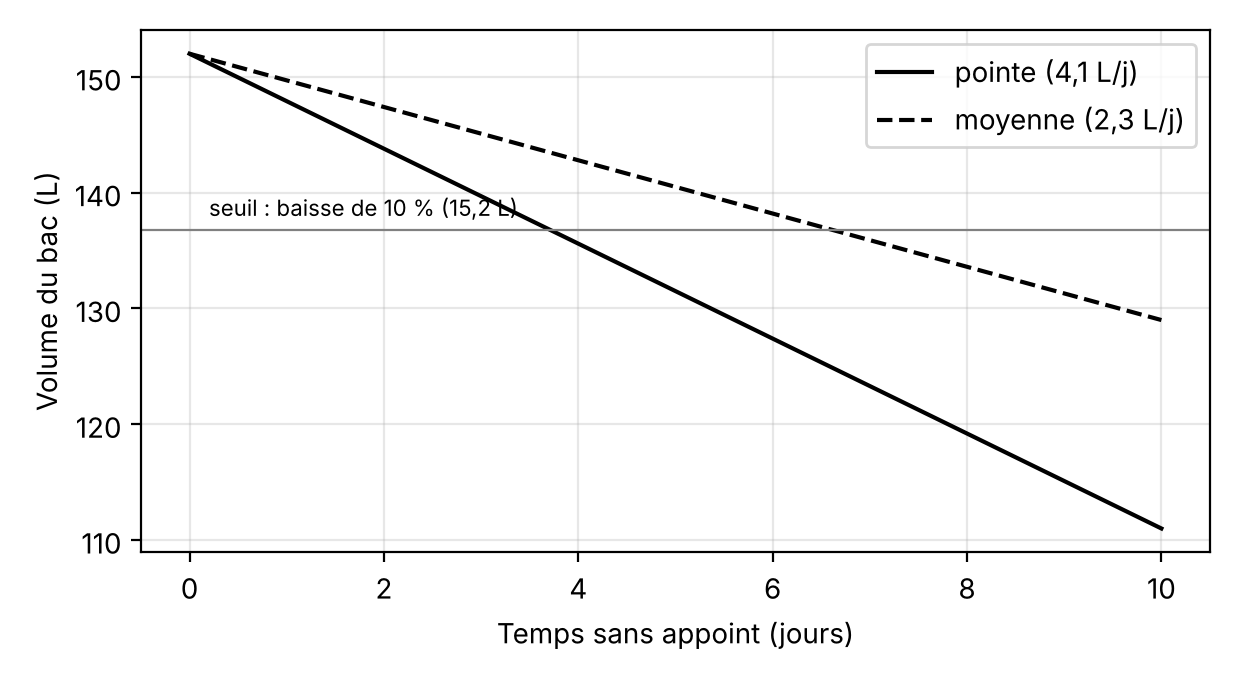
\includegraphics[width=0.78\textwidth]{img/bilan.png}
\caption{Volume du bac sans appoint, en pointe de consommation et en moyenne de cycle.}
\end{figure}

\naturecalc{théorie, avec les dimensions mesurées sur la tour (bac, flexible, tube) et des valeurs de fiches techniques ; aucun débit ni aucune consommation n'est mesuré}
\begin{demonstration}[effet d'une absence de deux semaines]
\resultat{EC_{14} \approx \qty{2,25}{mS/cm}}
Je note $V_{14}$ le volume consommé en $\qty{14}{j}$. En pointe :
\begin{align*}
V_{14} &= \qty{14}{j}\times\qty{4,1}{L/j}\\
V_{14} &= \qty{57,4}{L}
\end{align*}
En moyenne :
\begin{align*}
V_{14} &= \qty{14}{j}\times\qty{2,3}{L/j}\\
V_{14} &= \qty{32,2}{L}
\end{align*}
En pointe, il reste dans le bac $\qty{152}{L} - \qty{57,4}{L} = \qty{94,6}{L}$, soit une baisse de 38 \%. Dans le pire cas, les plants boivent l'eau sans prélever d'engrais : la même quantité de sels se retrouve dans un volume plus petit. La conductivité $EC$, en millisiemens par centimètre, est proportionnelle à la concentration en sels, donc inversement proportionnelle au volume :
\begin{align*}
EC_{14} &= EC_0\times\frac{V}{V - V_{14}}\\
EC_{14} &= \qty{1,4}{mS/cm}\times\frac{\qty{152}{L}}{\qty{94,6}{L}}\\
EC_{14} &\approx \qty{2,25}{mS/cm}
\end{align*}
\end{demonstration}

Une absence de deux semaines sans appoint dépasse donc la tolérance de 10 \%. Elle n'est acceptable qu'en début de cycle, quand les plants sont petits, ou en remplissant le bac au maximum avant le départ. En pointe de consommation, il faut un passage pour l'appoint au moins tous les trois à quatre jours.

\newcommand{\srcl}[2]{\href{#2}{\textcolor{blue}{\underline{#1}}}}

\subsection{Les besoins des plantes au cours de leur vie}

Les hypothèses du bilan hydrique (\qty{0,15}{L/j} en moyenne et \qty{0,30}{L/j} en pointe par plant) viennent de mon estimation. Je cherche ici à les vérifier avec la littérature : combien d'eau et de nutriments une laitue consomme-t-elle entre sa mise en tour et sa récolte, et comment cette consommation évolue-t-elle ? Je commence par la durée du cycle, puis je traite l'eau, puis les nutriments. Chaque chiffre de la littérature est suivi de sa source, cliquable : un clic ouvre la page du document. Les sources sont proposées pour validation, et la liste complète est à la fin de cette sous-partie.

\subsubsection*{La durée du cycle et la taille d'une laitue}

Une laitue hydroponique passe en moyenne \qty{30}{jours} de la mise en place du plant à la récolte, pour une tête de 5 à 6 onces, soit environ \qty{140}{g} à \qty{170}{g} (source \srcl{K}{https://www.aces.edu/wp-content/uploads/2022/08/ANR-2903_GreenhouseLettuceProduction_072822L-G.pdf}). Dans une chambre de culture fermée, des laitues cultivées en hydroponie jusqu'à \qty{28}{jours} après le semis ont atteint \qty{129}{g} à \qty{183}{g} de masse fraîche par plant (source \srcl{H}{https://journals.ashs.org/downloadpdf/view/journals/jashs/119/3/article-p610.pdf}). Une étude de modélisation retient \qty{144,6}{g} par plant et un cycle de \qty{30}{jours} (source \srcl{C}{https://www.mdpi.com/1660-4601/12/6/6879}). Je garde pour la tour un cycle de \qty{32}{jours} après la mise en tour, découpé en trois stades : la reprise (jours 0 à 5), la croissance des feuilles (jours 5 à 22) et la pommaison (jours 22 à 32). C'est la durée que j'ai retenue pour le suivi des plantes (partie 13).

\subsubsection*{L'eau consommée}

Une laitue consomme très peu d'eau au début, quand elle n'a que quelques feuilles, et de plus en plus ensuite : l'évapotranspiration d'un peuplement de laitues suit la surface de feuilles, et atteint son maximum à la récolte (source \srcl{H}{https://journals.ashs.org/downloadpdf/view/journals/jashs/119/3/article-p610.pdf}). Je traduis cela par un modèle simple : la consommation par plant, notée $c$ (en litres par jour), augmente linéairement avec le temps $t$ (en jours après la mise en tour), de zéro à sa valeur finale $c_f$ au jour $T = \qty{32}{j}$.

\naturecalc{théorie, à partir de valeurs tirées de la littérature ; rien de mesuré sur la tour}
\begin{demonstration}[eau consommée par une laitue pendant son cycle]
\resultat{W(T) = \frac{c_f\,T}{2} = \qty{4,8}{L}}
Je pose $c(t) = k\,t$, avec $k$ la pente de la droite, en litres par jour et par jour. La valeur finale vaut $c_f = k\,T$, donc :
\begin{align*}
k &= \frac{c_f}{T}\\
k &= \frac{\qty{0,30}{L/j}}{\qty{32}{j}}\\
k &= \qty{0,009375}{L/j^2}
\end{align*}
Le volume d'eau consommé entre le jour $0$ et le jour $t$, noté $W(t)$ en litres, est l'aire sous la droite, c'est-à-dire l'intégrale de $c$ :
\begin{align*}
W(t) &= \int_0^{t} k\,s\,\mathrm{d}s\\
W(t) &= \frac{k\,t^{2}}{2}
\end{align*}
En $t = T$, en remplaçant $k$ par $c_f/T$ :
\begin{align*}
W(T) &= \frac{c_f}{T}\times\frac{T^{2}}{2}\\
W(T) &= \frac{c_f\,T}{2}\\
W(T) &= \frac{\qty{0,30}{L/j}\times\qty{32}{j}}{2}\\
W(T) &= \qty{4,8}{L}
\end{align*}
La consommation moyenne sur le cycle est donc $W(T)/T = c_f/2 = \qty{0,15}{L/j}$ : c'est exactement mon hypothèse de départ, la moitié de la valeur de pointe.
\end{demonstration}

Je calcule maintenant ce que boit la laitue à chaque stade. À la fin de chaque stade, la consommation vaut $c = k\,t$ et le volume cumulé vaut $W = k\,t^{2}/2$.

\naturecalc{théorie, à partir de valeurs tirées de la littérature ; rien de mesuré sur la tour}
\begin{demonstration}[eau consommée à chaque stade]
\resultat{W_1 \approx \qty{0,12}{L},\quad W_2 \approx \qty{2,15}{L},\quad W_3 \approx \qty{2,53}{L}}
Avec $k = \qty{0,009375}{L/j^2}$, aux jours $t = 5$, $22$ et $32$ :
\begin{align*}
W(5) &= \frac{\qty{0,009375}{L/j^2}\times(\qty{5}{j})^{2}}{2} = \frac{\qty{0,009375}{L/j^2}\times\qty{25}{j^2}}{2} \approx \qty{0,117}{L}\\
W(22) &= \frac{\qty{0,009375}{L/j^2}\times(\qty{22}{j})^{2}}{2} = \frac{\qty{0,009375}{L/j^2}\times\qty{484}{j^2}}{2} \approx \qty{2,269}{L}\\
W(32) &= \frac{\qty{0,009375}{L/j^2}\times(\qty{32}{j})^{2}}{2} = \frac{\qty{0,009375}{L/j^2}\times\qty{1024}{j^2}}{2} = \qty{4,8}{L}
\end{align*}
Le volume de chaque stade est la différence des volumes cumulés :
\begin{align*}
W_1 &= W(5) - W(0) \approx \qty{0,117}{L} - \qty{0}{L} = \qty{0,117}{L}\\
W_2 &= W(22) - W(5) \approx \qty{2,269}{L} - \qty{0,117}{L} = \qty{2,152}{L}\\
W_3 &= W(32) - W(22) \approx \qty{4,8}{L} - \qty{2,269}{L} = \qty{2,531}{L}
\end{align*}
Les consommations en fin de stade valent $c(5) = \qty{0,009375}{L/j^2}\times\qty{5}{j} \approx \qty{0,047}{L/j}$ et $c(22) = \qty{0,009375}{L/j^2}\times\qty{22}{j} \approx \qty{0,206}{L/j}$.
\end{demonstration}

Le tableau suivant donne l'eau consommée par une laitue à chaque stade, avec un modèle linéaire.

\begin{table}[H]
\centering
\small
\renewcommand{\arraystretch}{1.1}
\begin{tabularx}{\textwidth}{|>{\raggedright\arraybackslash}p{4.4cm}|Y|Y|Y|Y|}
\hline
\textbf{Stade} & \textbf{Jours} & \textbf{$c$ en fin de stade (\unit{L/j})} & \textbf{Eau du stade (\unit{L})} & \textbf{Part du cycle} \\
\hline
Reprise & 0 à 5 & 0,047 & 0,12 & \qty{2}{\percent} \\
\hline
Croissance des feuilles & 5 à 22 & 0,206 & 2,15 & \qty{45}{\percent} \\
\hline
Pommaison & 22 à 32 & 0,300 & 2,53 & \qty{53}{\percent} \\
\hline
\textbf{Cycle entier} & 0 à 32 & 0,300 & \textbf{4,80} & \qty{100}{\percent} \\
\hline
\end{tabularx}
\caption{Eau consommée par une laitue à chaque stade (modèle linéaire, valeurs de calcul).}
\end{table}

Plus de la moitié de l'eau est bue pendant les dix derniers jours : c'est là que la tour demande le plus au bac, et c'est donc le cas que je retiens pour dimensionner l'appoint. Pour les 12 plants, le cycle consomme $12 \times \qty{4,8}{L} = \qty{57,6}{L}$, auxquels s'ajoutent $\qty{32}{j} \times \qty{0,5}{L/j} = \qty{16}{L}$ d'évaporation, soit \qty{73,6}{L}, environ la moitié du volume du bac de \qty{152}{L}.

Je compare ce modèle à la littérature. Pour une laitue de \qty{150}{g} à \qty{250}{g} en hydroponie, la solution consommée va de \qty{3}{L} à \qty{6}{L} par plant, et une laitue de \qty{200}{g} en consomme environ \qty{3}{L} à \qty{4}{L}, à Hawaï, un climat tropical proche de celui de la Polynésie (source \srcl{J}{https://www.ctahr.hawaii.edu/Hawaii/downloads/Three_Non-circulating_Hydroponic_Methods_for_Growing_lettuce.pdf}). La modélisation de la source \srcl{C}{https://www.mdpi.com/1660-4601/12/6/6879} donne \qty{20}{L} d'eau par kilogramme de laitue : pour une tête de \qty{0,1446}{kg}, cela fait $\qty{20}{L/kg}\times\qty{0,1446}{kg} \approx \qty{2,9}{L}$ par plant. Enfin, à pleine canopée, le peuplement de la source \srcl{H}{https://journals.ashs.org/downloadpdf/view/journals/jashs/119/3/article-p610.pdf} évapotranspire environ \qty{4}{L/(m^2.j)} ; comme il compte environ 18 à 19 plants par mètre carré (surface de \qty{20}{m^2} supposée), cela fait $\qty{4}{L/(m^2.j)}$ divisés par 19 plants par mètre carré, soit $\qty{4}{L/(m^2.j)}/19 \approx \qty{0,21}{L/j}$ par plant au moment de la récolte. Mon modèle (\qty{4,8}{L} par cycle et \qty{0,30}{L/j} à la fin) est donc dans la fourchette haute de la littérature, ce qui est volontaire : une hypothèse trop forte sur la consommation d'eau protège le dimensionnement de l'appoint, alors qu'une hypothèse trop faible le mettrait en défaut.

\subsubsection*{Les nutriments consommés}

Une laitue prélève surtout de l'azote (N), du phosphore (P) et du potassium (K), et beaucoup moins de calcium (Ca) et de magnésium (Mg). Une étude brésilienne qui a suivi la croissance de laitues hydroponiques pendant \qty{30}{jours} après la mise en place mesure, à la fin, \qty{295,4}{mg} d'azote, \qty{31,9}{mg} de phosphore et \qty{641,7}{mg} de potassium par plant (source \srcl{L}{https://doaj.org/article/3cad1b7f657c4b9897b2eca48a74d30d}). Pour le calcium et le magnésium, la source \srcl{H}{https://journals.ashs.org/downloadpdf/view/journals/jashs/119/3/article-p610.pdf} donne les concentrations dans les feuilles, ce qui permet de recalculer une quantité par plant à partir de la masse sèche.

\naturecalc{théorie, à partir de valeurs tirées de la littérature ; rien de mesuré sur la tour}
\begin{demonstration}[nutriments contenus dans une laitue à la récolte]
\resultat{m_{N} \approx \qty{383}{mg},\quad m_{P} \approx \qty{32}{mg},\quad m_{K} \approx \qty{1294}{mg},\quad m_{Ca} \approx \qty{79}{mg},\quad m_{Mg} \approx \qty{25}{mg}}
Pour un élément, la masse $m$ contenue dans une plante, en milligrammes, est la concentration $x$ de cet élément dans la matière sèche, en milligrammes par gramme, multipliée par la masse sèche $M_s$ de la plante, en grammes :
\begin{align*}
m &= x \times M_s
\end{align*}
La source \srcl{H}{https://journals.ashs.org/downloadpdf/view/journals/jashs/119/3/article-p610.pdf} donne $M_s = \qty{8,8}{g}$ par plant (pour \qty{183}{g} de masse fraîche) et, pour les concentrations, \qty{43500}{\micro g/g} d'azote, \qty{3630}{\micro g/g} de phosphore, \qty{147000}{\micro g/g} de potassium, \qty{9000}{\micro g/g} de calcium et \qty{2890}{\micro g/g} de magnésium. Comme $\qty{1}{mg} = \qty{1000}{\micro g}$, on a par exemple $\qty{43500}{\micro g/g} = \qty{43,5}{mg/g}$. Je calcule élément par élément :
\begin{align*}
m_{N} &= \qty{43,5}{mg/g}\times\qty{8,8}{g} \approx \qty{383}{mg}\\
m_{P} &= \qty{3,63}{mg/g}\times\qty{8,8}{g} \approx \qty{31,9}{mg}\\
m_{K} &= \qty{147}{mg/g}\times\qty{8,8}{g} \approx \qty{1294}{mg}\\
m_{Ca} &= \qty{9,0}{mg/g}\times\qty{8,8}{g} \approx \qty{79,2}{mg}\\
m_{Mg} &= \qty{2,89}{mg/g}\times\qty{8,8}{g} \approx \qty{25,4}{mg}
\end{align*}
Ce sont des estimations : les concentrations viennent des feuilles et d'un autre cultivar que celui de la tour.
\end{demonstration}

Les deux sources donnent le même ordre de grandeur pour l'azote et la même valeur pour le phosphore ; elles diffèrent d'un facteur deux pour le potassium, ce qui n'a rien d'étonnant entre deux cultivars et deux systèmes. Je retiens donc une fourchette. Pour 12 plants, et en divisant par les \qty{30}{jours} de l'étude brésilienne, on obtient les besoins suivants.

\begin{table}[H]
\centering
\small
\renewcommand{\arraystretch}{1.1}
\begin{tabularx}{\textwidth}{|>{\raggedright\arraybackslash}p{2.6cm}|Y|Y|Y|}
\hline
\textbf{Élément} & \textbf{Par plant, sur le cycle (\unit{mg})} & \textbf{Par plant, par jour (\unit{mg/j})} & \textbf{12 plants, sur le cycle (\unit{g})} \\
\hline
Azote (N) & 295 à 383 & 9,8 à 12,8 & 3,5 à 4,6 \\
\hline
Phosphore (P) & 32 & 1,1 & 0,38 \\
\hline
Potassium (K) & 642 à 1294 & 21 à 43 & 7,7 à 15,5 \\
\hline
Calcium (Ca) & 79 & 2,6 & 0,95 \\
\hline
Magnésium (Mg) & 25 & 0,85 & 0,31 \\
\hline
\end{tabularx}
\caption{Nutriments prélevés par une laitue sur un cycle, d'après les sources L et H, et besoins des 12 plants.}
\end{table}

Pour savoir si le bac contient assez de nutriments pour tout un cycle, je compare ces besoins à ce que le bac contient quand la solution est bien réglée. Une étude de 2025 sur la laitue hydroponique fixe, pour la laitue Bibb, l'équilibre idéal à \qty{132}{mg/L} d'azote, \qty{35}{mg/L} de phosphore et \qty{174}{mg/L} de potassium (source \srcl{M}{https://doaj.org/article/3f4baf90f7064b70be9ff31b0bc3bfbc}).

\naturecalc{théorie, à partir de valeurs tirées de la littérature ; rien de mesuré sur la tour}
\begin{demonstration}[part des nutriments du bac prélevée par les 12 plants]
\resultat{\text{azote : } \qty{18}{\percent} \text{ à } \qty{23}{\percent}\quad\text{et potassium : } \qty{29}{\percent} \text{ à } \qty{59}{\percent}}
La masse d'un élément dans le bac, notée $m_{bac}$ en milligrammes, est sa concentration $\rho$, en milligrammes par litre, multipliée par le volume $V = \qty{152}{L}$ :
\begin{align*}
m_{bac} &= \rho\times V\\
m_{bac,N} &= \qty{132}{mg/L}\times\qty{152}{L} = \qty{20064}{mg}\\
m_{bac,P} &= \qty{35}{mg/L}\times\qty{152}{L} = \qty{5320}{mg}\\
m_{bac,K} &= \qty{174}{mg/L}\times\qty{152}{L} = \qty{26448}{mg}
\end{align*}
La part prélevée par les 12 plants est le rapport de leur besoin au contenu du bac. Pour l'azote, avec les valeurs non arrondies \qty{3545}{mg} (environ \qty{3,5}{g}) et \qty{4594}{mg} (environ \qty{4,6}{g}) :
\begin{align*}
\frac{\qty{3545}{mg}}{\qty{20064}{mg}} &\approx \qty{17,7}{\percent}\\
\frac{\qty{4594}{mg}}{\qty{20064}{mg}} &\approx \qty{22,9}{\percent}
\end{align*}
Pour le phosphore, $\qty{383}{mg}/\qty{5320}{mg} \approx \qty{7,2}{\percent}$. Pour le potassium, avec $\qty{7700}{mg}$ et $\qty{15523}{mg}$ :
\begin{align*}
\frac{\qty{7700}{mg}}{\qty{26448}{mg}} &\approx \qty{29,1}{\percent}\\
\frac{\qty{15523}{mg}}{\qty{26448}{mg}} &\approx \qty{58,7}{\percent}
\end{align*}
\end{demonstration}

Le bac de \qty{152}{L} contient donc, quand il est bien réglé, beaucoup plus d'éléments nutritifs que les 12 plants n'en prélèvent en un cycle : de \qty{7}{\percent} à \qty{59}{\percent} selon l'élément. Ce résultat concorde avec une étude de l'université de Floride sur la laitue en film nutritif : seule une petite fraction des éléments apportés finit dans la plante (\qty{12,1}{\percent} de l'azote, \qty{12,6}{\percent} du phosphore, \qty{20,3}{\percent} du potassium), et les teneurs en azote, phosphore et calcium de la solution étaient plus élevées en fin d'essai qu'au début (source \srcl{N}{https://edis.ifas.ufl.edu/publication/AE610/pdf}). Cela a deux conséquences pour la tour. D'abord, le dosage ne sert pas à reconstituer la totalité des nutriments consommés : il corrige de petites dérives de l'EC, ce qui explique les doses de quelques millilitres des pompes -M2 et -M3. Ensuite, la conductivité monte surtout quand l'eau disparaît (consommation et évaporation) et que les sels restent : c'est le phénomène que j'étudie dans la sous-partie suivante.

\begin{aretenir}
Une laitue boit environ \qty{4,8}{L} d'eau pendant son cycle de \qty{32}{jours}, plus de la moitié pendant les dix derniers jours, et prélève de l'ordre de \qty{300}{mg} à \qty{400}{mg} d'azote, \qty{32}{mg} de phosphore et \qty{640}{mg} à \qty{1300}{mg} de potassium. Ces valeurs viennent de la littérature (cultivars et systèmes différents du mien) : elles donnent l'ordre de grandeur, et seules les mesures de la tour les confirmeront.
\end{aretenir}

\subsection{Pourquoi je n'ajoute pas de bac de secours}

Dans la première version de l'étude, la tour comportait un bac de secours d'eau claire, une pompe d'appoint (P5) et un second ruban de niveau pour remplir le bac principal automatiquement. Dans la version actuelle, j'ai supprimé ces trois éléments : l'appoint se fait à la main, avec un seau. Je justifie ici ce choix, parce qu'un bac de secours paraît de bon sens : il faut regarder ce qu'il apporte réellement, et ce qu'il coûte.

\subsubsection*{Ce qu'un bac de secours résoudrait}

Un bac de secours ne résout qu'un seul problème : le bac principal baisse de niveau et sa solution se concentre quand personne ne peut ajouter d'eau. La question est donc de savoir combien de temps la tour tient sans appoint. Dans le pire cas (les plants boivent l'eau mais ne prélèvent pas de sels, comme dans la sous-partie précédente), la conductivité vaut $EC = EC_0\,V/(V - V_c)$, avec $V_c$ le volume consommé. J'impose une limite à cette conductivité et j'en déduis la durée. Je prends deux limites : le haut de la plage cible de la laitue, \qty{1,8}{mS/cm}, et le seuil d'alarme du dashboard, \qty{2,2}{mS/cm} (à partir duquel la laitue risque des pointes brûlées).

\naturecalc{théorie, avec les dimensions mesurées sur la tour (bac, flexible, tube) et des valeurs de fiches techniques ; aucun débit ni aucune consommation n'est mesuré}
\begin{demonstration}[durée sans appoint selon la conductivité tolérée]
\resultat{T = \frac{V}{C}\left(1 - \frac{EC_0}{EC_{lim}}\right)}
Je pars de la relation $EC_{lim} = EC_0\,V/(V - V_c)$, où $EC_0 = \qty{1,4}{mS/cm}$ est la conductivité de départ, $EC_{lim}$ la limite tolérée, $V = \qty{152}{L}$ le volume du bac et $V_c$ le volume consommé, en litres. Je l'isole ligne par ligne :
\begin{align*}
EC_{lim}\,(V - V_c) &= EC_0\,V\\
V - V_c &= V\,\frac{EC_0}{EC_{lim}}\\
V_c &= V\left(1 - \frac{EC_0}{EC_{lim}}\right)
\end{align*}
La consommation journalière $C$ étant constante (en litres par jour), $V_c = C\,T$, d'où le résultat. Pour la limite de \qty{1,8}{mS/cm} :
\begin{align*}
V_c &= \qty{152}{L}\times\left(1 - \frac{\qty{1,4}{mS/cm}}{\qty{1,8}{mS/cm}}\right)\\
V_c &= \qty{152}{L}\times0{,}2222\\
V_c &\approx \qty{33,8}{L}
\end{align*}
\begin{align*}
T_{pic} &= \frac{\qty{33,8}{L}}{\qty{4,1}{L/j}} \approx \qty{8,2}{j}\\
T_{moy} &= \frac{\qty{33,8}{L}}{\qty{2,3}{L/j}} \approx \qty{14,7}{j}
\end{align*}
Pour la limite de \qty{2,2}{mS/cm} :
\begin{align*}
V_c &= \qty{152}{L}\times\left(1 - \frac{\qty{1,4}{mS/cm}}{\qty{2,2}{mS/cm}}\right)\\
V_c &= \qty{152}{L}\times0{,}3636\\
V_c &\approx \qty{55,3}{L}
\end{align*}
\begin{align*}
T_{pic} &= \frac{\qty{55,3}{L}}{\qty{4,1}{L/j}} \approx \qty{13,5}{j}\\
T_{moy} &= \frac{\qty{55,3}{L}}{\qty{2,3}{L/j}} \approx \qty{24,0}{j}
\end{align*}
\end{demonstration}

Les trois critères donnent donc les autonomies suivantes, sans aucun appoint.

\begin{table}[H]
\centering
\small
\renewcommand{\arraystretch}{1.1}
\begin{tabularx}{\textwidth}{|>{\raggedright\arraybackslash}p{6.4cm}|Y|Y|}
\hline
\textbf{Critère} & \textbf{En pointe (\unit{j})} & \textbf{En moyenne (\unit{j})} \\
\hline
Baisse de \qty{10}{\percent} du volume (prudent) & 3,7 & 6,6 \\
\hline
$EC$ atteint \qty{1,8}{mS/cm} (haut de la plage cible) & 8,2 & 14,7 \\
\hline
$EC$ atteint \qty{2,2}{mS/cm} (alarme) & 13,5 & 24,0 \\
\hline
\end{tabularx}
\caption{Durée sans appoint selon le critère retenu, avec $EC_0 = \qty{1,4}{mS/cm}$.}
\end{table}

\naturecalc{théorie, avec les dimensions mesurées sur la tour (bac, flexible, tube) et des valeurs de fiches techniques ; aucun débit ni aucune consommation n'est mesuré}
\begin{demonstration}[conductivité après une absence d'une semaine ou de deux semaines]
\resultat{EC_{7} \approx \qty{1,73}{mS/cm}\quad\text{et}\quad EC_{14} \approx \qty{2,09}{mS/cm}}
Une semaine entièrement en pointe consomme $V_c = \qty{7}{j}\times\qty{4,1}{L/j} = \qty{28,7}{L}$. Avec la relation $EC = EC_0\,V/(V - V_c)$ :
\begin{align*}
EC_{7} &= \qty{1,4}{mS/cm}\times\frac{\qty{152}{L}}{\qty{152}{L} - \qty{28,7}{L}}\\
EC_{7} &= \qty{1,4}{mS/cm}\times\frac{\qty{152}{L}}{\qty{123,3}{L}}\\
EC_{7} &\approx \qty{1,73}{mS/cm}
\end{align*}
La pointe ne dure que les dix derniers jours du cycle. Deux semaines au pire moment du cycle comptent donc au plus dix jours de pointe et quatre jours de consommation moyenne :
\begin{align*}
V_c &= \qty{10}{j}\times\qty{4,1}{L/j} + \qty{4}{j}\times\qty{2,3}{L/j}\\
V_c &= \qty{41,0}{L} + \qty{9,2}{L} = \qty{50,2}{L}
\end{align*}
\begin{align*}
EC_{14} &= \qty{1,4}{mS/cm}\times\frac{\qty{152}{L}}{\qty{152}{L} - \qty{50,2}{L}}\\
EC_{14} &= \qty{1,4}{mS/cm}\times\frac{\qty{152}{L}}{\qty{101,8}{L}}\\
EC_{14} &\approx \qty{2,09}{mS/cm}
\end{align*}
\end{demonstration}

Même dans le pire cas, une absence d'une semaine laisse la conductivité dans la plage cible (\qty{1,73}{mS/cm}, sous \qty{1,8}{mS/cm}), et une absence de deux semaines, au pire moment du cycle, reste sous le seuil d'alarme (\qty{2,09}{mS/cm}, sous \qty{2,2}{mS/cm}). La règle de \qty{10}{\percent} de la sous-partie précédente est donc très prudente : elle fixe la fréquence confortable des passages, pas la limite de ce que la tour supporte. Et ce calcul prend le pire cas, où les plants ne prélèvent aucun sel : en réalité, ils en prélèvent une partie, et la conductivité monte moins vite.

\subsubsection*{Pourquoi cela ne justifie pas un bac de secours}

Un bac de secours de volume $V_s$ allonge l'autonomie de $V_s/C$ : avec \qty{40}{L}, cela fait $\qty{40}{L}/\qty{4,1}{L/j} \approx \qty{9,8}{j}$ en pointe. Mais ce bac de secours doit lui-même être rempli à la main, et c'est là son premier défaut : il ne supprime pas le geste d'aller chercher de l'eau, il le repousse. Or ce geste est léger. En pointe, la tour consomme \qty{4,1}{L/j}, soit un seau de \qty{10}{L} tous les deux jours et demi, ou trois seaux par semaine. Et la tour est visitée, puisque je mesure, je règle et j'entretiens : le projet est un démonstrateur suivi régulièrement, pas un système laissé seul plusieurs semaines.

Le deuxième défaut est la fiabilité. Un remplissage automatique ajoute des pannes possibles : un ruban de niveau qui se décale, une pompe d'appoint qui reste enclenchée ou qui ne démarre plus. Une pompe bloquée en marche remplit le bac jusqu'au débordement, car le système n'a aucun moyen d'évacuer l'excédent, et le bac contient une solution nutritive qu'il ne faut pas rejeter. Un ruban faussé qui déclenche trop d'appoint dilue la solution : le dosage ne sait pas retirer de l'eau, il ne sait qu'ajouter des engrais. Avec l'appoint manuel, c'est une personne qui décide, et elle regarde le niveau et la conductivité avant d'ajouter de l'eau.

Le troisième défaut est le nombre de pièces. Le bac de secours demande un second réservoir, une pompe, un second ruban de niveau avec son entrée sur le convertisseur analogique-numérique, une sortie de la carte MOSFET\ix{15}, un fusible, des câbles, du programme et des essais en plus : chacun de ces éléments est à acheter, à câbler et à tester, dans un projet où je dois condenser trois années de formation en trois mois. Il touche aussi le bilan d'énergie : j'ai retiré la pompe d'appoint du bilan de la partie 5, où chaque wattheure compte pour que le panneau et les batteries restent dimensionnés avec une marge.

Enfin, le système protège déjà ce que le bac de secours protégerait. Quand le réservoir passe sous \qty{15}{\percent}, le pilote arrête la pompe et le dosage et lève une alarme « ajouter de l'eau » (partie 8.4), et, dans la première version du programme (partie 8.12), l'Arduino coupait lui-même la circulation sous le seuil de niveau. Dans la version actuelle, cette décision est prise par le Raspberry, et la coupure de l'Arduino après \qty{30}{s} de silence ne mesure pas le niveau : une protection locale contre la marche à sec reste à ajouter dans l'Arduino (partie 8.3). Quand la conductivité devient trop haute, la règle de décision du pilote recommande d'ajouter de l'eau claire. La tour s'arrête donc dans un état sûr, et le dashboard me prévient : la seule chose qu'elle ne fait pas est de se remplir toute seule.

\begin{aretenir}
Sans aucun appoint, la tour tient au moins une semaine au pire moment du cycle dans la plage cible de conductivité (\qty{1,73}{mS/cm}) et deux semaines sous le seuil d'alarme (\qty{2,09}{mS/cm}). Un bac de secours ne ferait que repousser le remplissage à la main, ajouterait des pannes possibles (débordement, dilution) et des pièces à acheter, câbler et tester, et alourdirait le bilan d'énergie. Je garde donc un bac unique et un appoint manuel, avec un passage tous les trois à quatre jours en pointe. Je reconsidérerai ce choix si la tour devait rester sans visite plus de deux semaines pendant la pointe : un remplissage par flotteur mécanique, sans pompe, serait alors la première solution à étudier.
\end{aretenir}

\subsubsection*{Sources de cette sous-partie}

Les sources C, H, J, K, L, M et N de cette sous-partie sont dans la bibliographie, à la toute fin du rapport. Dans le texte, chaque lettre est un lien cliquable vers la page de la source.

\subsection{Protocole de mesure}

Aucune mesure n'est encore faite : tout ce qui précède vient de la fiche de la pompe, du plan du couvercle et d'hypothèses. Les mesures suivantes permettront de remplacer les hypothèses par des valeurs réelles. Pour toutes, il faut un seau gradué de \qty{10}{L}, un chronomètre et un mètre ruban.

Pour le \textbf{débit réel de la pompe}, je garde le circuit complet (couvercle répartiteur en place, flexible raccordé), car c'est le point de fonctionnement calculé. Je place le seau gradué au pied de la tour et je recueille toute l'eau qui retombe de la paroi. Je démarre la pompe, j'attends \qty{10}{s} que le débit se stabilise, puis je lance le chronomètre et je l'arrête quand le seau atteint \qty{10}{L}. Je reverse l'eau dans le bac et je recommence cinq fois. Un second essai, flexible débranché du couvercle et sortie à \qty{1,2}{m} au-dessus de l'eau, donne le débit sans les pertes du couvercle et permet de les isoler. Le débit en litres par heure est $Q = 3600\,V_s/t$, avec $V_s$ le volume du seau, en litres, et $t$ la durée, en secondes. La valeur attendue est \qty{388}{L/h}.

Pour la \textbf{hauteur du jet}, je retire le couvercle, j'oriente l'extrémité du flexible vers le haut et je fixe un mètre ruban à la verticale. Je photographie le jet cinq fois et je relève sa hauteur maximale. Sans frottement de l'air, elle devrait être proche de \qty{15}{cm} pour l'ensemble des huit trous ; avec le flexible seul, la hauteur dépend de la section de sortie, donc cette mesure sert surtout à comparer deux essais entre eux.

Pour la \textbf{répartition de l'eau}, qui est la difficulté de départ, je fais tourner la pompe avec le couvercle en place et je regarde la paroi : les huit zones arrosées doivent se rejoindre, sans zone sèche entre elles. Je note aussi le nombre de godets dont les racines sont mouillées.

Pour la \textbf{consommation d'eau}, je colle une règle graduée verticale dans le bac. Chaque jour à la même heure, pompe arrêtée depuis plus de cinq minutes, je relève la hauteur d'eau, et je note les appoints mesurés au seau. Après au moins sept jours, la pente de la droite du niveau en fonction du temps donne la consommation en litres par jour, à comparer à \qty{2,3}{L/j} en moyenne et \qty{4,1}{L/j} en pointe.

\begin{aretenir}
La pompe de \qty{800}{L/h} débite environ \qty{388}{L/h} dans le circuit, sous \qty{2,57}{m} : c'est le flexible de \qty{9}{mm} qui limite le débit, non le couvercle. Le débit moyen est d'environ \qty{32}{L/h} par plant, soit 16 fois le besoin minimal retenu (à confirmer par la mesure de répartition), et le bac de \qty{152}{L} se renouvelle en \qty{23,5}{min}. Le bac consomme \qty{2,3}{L/j} en moyenne et \qty{4,1}{L/j} en pointe : il faut un appoint d'environ \qty{15}{L} tous les quatre jours en pointe. Ces chiffres sont théoriques tant que les mesures ne sont pas faites.
\end{aretenir}


